\section{Building Practical Multithreaded SMR System} \label{sec:crane-plan}

This section proposes the preliminary design of \crane. As this project moves
forward and our case study goes broadly, significant refinements on the design
will be necessary. In the following sections, we will introduce the architecture
of \crane with its components (\S~\ref{sec:rep-arch}), describe our new
algorithm that addresses the request timing challenge across replicas
(\S~\ref{sec:rep-time-algo}), present our checkpoint scheme for critical program
states (\S~\ref{sec:rep-checkpoint}), identify various implementation-level
challenges (\S~\ref{sec:rep-impl}), and describe our comprehensive case study
plan (\S~\ref{sec:rep-eval}). 

\begin{figure}[t]
\centering
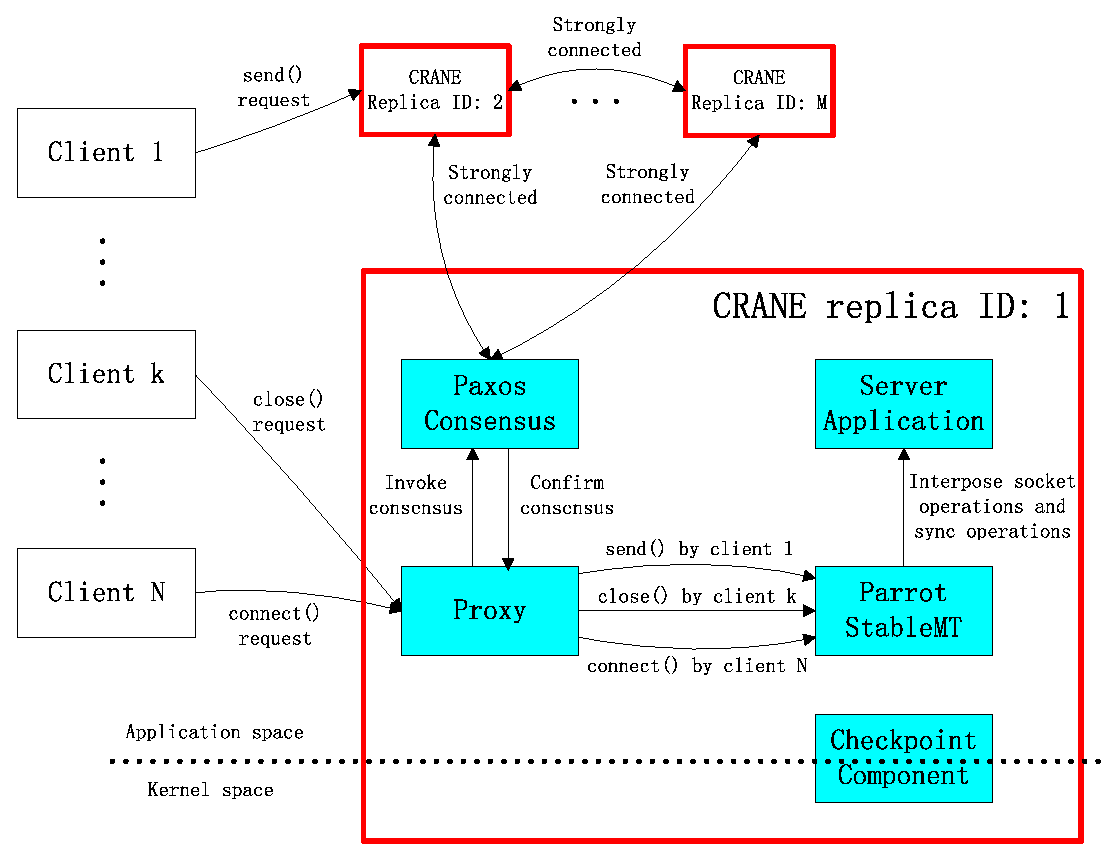
\includegraphics[width=0.67\columnwidth]{figures/architecture}
\vspace{-.05in}
\caption{{\em The \crane architecture Design.}} \label{fig:arch}
\vspace{-.05in}
\end{figure}

\subsection{\crane Architecture Design} \label{sec:rep-arch}

\crane uses a static replica configuration: each replica has its own unique
replica ID, and the set of replicas in the \crane system never changes. More
specifically, some replicas can go down forever, but no new replica will join
the system after \crane launches. Because \crane's main purpose is replicating
multithreaded applications, not general consistent distributed systems, we
consider this configuration realistic.
%% This configuration also greatly simplifies our system design.

Currently the \crane system design ignores the ``read only optimization" in some
modern SMR systems, and requires all replicas to process the same input
sequence. To make replicas reach consensus on a input request sequence, a SMR
system needs to define the request interface as the consensus objectives. Some
systems (\eg, ZooKeeper~\cite{zookeeper}) define their own file-system style
interface for consensus, but they are mainly designed for storage systems. In
order to support general multithreaded programs, especially real-world server
programs (\eg, web servers, SQL servers, and key-value store servers), \crane
proposes to choose the popular Linux socket operations (\eg, \connect, \accept,
\send, and \recv) as the request interface for consensus. We will discuss in
detail how \crane handles each socket operation in section~\S\ref{sec:rep-api}.

Figure~\ref{fig:arch} shows the high level architecture design of our \crane
system. It works as a typical client-server model with $N$ (can be tens or
hundreds) clients and $M$ (3 or 5 in a typical SMR setting) server replicas.
Each \crane replica has five components: (1) a consensus component; (2) a proxy
component; (3) a \smt runtime; (4) a replicated multithreaded server
application; and (5) a checkpoint component.

%%\crane has some default actions that conform to default SMR behaviors. 
In normal execution cases, when \crane starts, a replica will be elected as the
leader replica using consensus component. In addition, for each socket
operation, this leader will invoke a consensus message to the other replicas
through the consensus component. The consensus component implements a \paxos
distributed consensus protocol for all consensus requests, and all replicas'
consensus components will try to maintain a strong connection with each other.
The proxy component is a coordinator among the clients, the consensus component,
and the \smt runtime: a proxy accepts an input request from a client, asks for
consensus, and then sends this request to the \smt runtime. The \smt runtime and
the replicated multithreaded application are within the same process, and this
process is forked from the proxy component as a replica launches. We leverage
our prior work \parrot system as our \smt runtime because of its high
practicality. The \parrot runtime intercepts Pthreads synchronization operations
(\eg, \mutexlock) of the replicated multithreaded application, and avoids
divergent thread interleavings of this program by eliminating nondeterminism of
these synchronization operations.

To handle exceptional cases, including replica failures or network partitions,
the proxy persistently logs operations that have reached consensus. If a replica
fails and restarts, it can restore a consistent sequence of requests from this
log. If the leader fails, leader re-election is handled by the default \paxos
protocol in the consensus component. A checkpoint (\S\ref{sec:rep-checkpoint})
component sits on both the application side and kernel side in order to
checkpoint both the server application and the \smt runtime (both of which are
within the same process). We explicitly design the proxy to be stateless and it
needs no checkpoint. The consensus component does not need checkpoints either,
because it can recover requests from the operation log. Because a checkpoint
operation is expensive, \crane lets the leader incorporate a checkpoint
operation as a consensus request, and periodically assigns a random non-leader
replica ID to do this operation. Each checkpoint is stored in the local replica
and 
synchronized to other replicas when the system is not busy handling requests.
This design choice allows the leader replica to process requests normally
without slowing down the system, and each replica can still have persistent
checkpoints (not necessarily the latest checkpoints) for recovery.


\subsubsection{Handling Consensus Interface}  \label{sec:rep-api}

As mentioned in section~\ref{sec:rep-arch}, \crane chooses the popular Linux
socket operations (\eg, \connect, \accept, \send, and \recv) as the request
interface for consensus. We focus on replicating application states on the
server side, not the entire client-server system (\ie, \crane is not designed to
replicate the clients' execution states, and therefore does not need to handle
\send operations in the replicated server application). Therefore, \crane only
needs to support blocking socket operations at server side that depend on
external network inputs. Here is a list of popular blocking socket operations we
support: \recv, \sockread, \accept, \select, \poll, and \epoll. We expect that
these operations can already support a wide range of real-world multithreaded
server applications, and more operations can be easily added if necessary.

One critical challenge of reaching consensus for blocking socket operations is:
neither the proxy nor the \smt module can know what operations a server is going
to execute. We can not passively block all blocking operations on the server
side and then ask for consensus, because this may be too slow; we want to
perform consensus upfront and concurrently. Fortunately, each of these blocking
operations must correspond to an event on the ``client" side (in \crane, the
proxy is the client that sends requests to the server). On the proxy side, there
are only three operations interacting with the servers: \send, \connect, and
\close. Currently we classify all blocking operations on the server side into
two categories:

\textbf{(1) One sender and one receiver.} For instance, when the proxy sees a
\connect operation from the client, it invokes a consensus request with \accept.
The other instance is: when the proxy sees a \send operation from the client, it
invokes a consensus request with \recv. If no \select or \poll operation is
executed at runtime, then all operations in a replicated application are within
this category. Enforcing a consistent logical clock for operations across
replicas in this category is easy, and more details are given in
section~\S\ref{sec:rep-time-algo}.

\textbf{(2) Multiple senders and one receiver.} This category involves a single
\select or \poll and multiple \send or \connect operations. Let's take \select
as example, as handling \poll and \epoll are similar. Handling this category is
challenging because we we need to make sure 
all replicas execute the same sequence (including the same time values) of
\select operations with mixed use of \recv and \accept. For each \select
operation, we must ensure the same set of \send or \connect operations across
replicas. To address this challenge, we propose with a simple and effective
design: in this mode, we actually only need to handle \select, because in this
category, both \recv and \accept become non-blocking (so they do not need any
consensus and do not consume any logical clocks). In the proxy of the leader
replica, we batch up to $N$ \send or \connect operations until a timeout T in
the proxy occurs, and both N and T are configurable parameters in \crane. Then,
for each batch of these operations, we invoke a \paxos consensus request, and
incorporate these requests as the contents of the \paxos consensus operation,
which ensures that all replicas run the same batch of requests. 

\subsubsection{Deployment Requirements and Guarantees} 
\label{sec:rep-discussion}

\crane guarantees the same fault-tolerance strength as those common SMR systems
built on top of \paxos because our consensus interface carries all parameters of
the socket operations as part of the value of each \paxos consensus instance,
which conforms to a default \paxos protocol. As a result, as long as more than
half of replicas in \crane still behave normally, \crane is still available to
users.

Unlike \parrot that ignores data races, \crane requires no fundamental
assumptions on multithreading concurrency. This is because we can leverage the
\crane replication architecture to run a race detector on a dedicated non-leader
replica, which can detect races at runtime for developer diagnosis. \crane only
requires that applications be Pthreads-compatible, x86 binary, and use socket
operations to accept requests.

% \crane assumes a stateless OS kernel, because it performs application-level
% program checkpoints. This assumption is common in existing SMR systems. In
order % to handle minor systems resources divergence such as file descriptors,
\crane % does a internal mapping between  \S~\ref{}


\subsection{The Timing Handling Algorithm} \label{sec:rep-time-algo}
This section first introduces some primitives in our \parrot \smt runtime, and
then describes our timing handling algorithm design. These \parrot primitives
are necessary on understanding challenges and our solutions for the \smt and SMR
integration.

\subsubsection{Introduction to the \parrot \smt System} \label{sec:rep-parrot}
\parrot is a pure runtime system that uses a Linux technique called \ldpreload
to interpose Pthreads synchronizations (\eg, \mutexlock), and to enforce a
deterministic total order for these synchronization operations at runtime,
greatly reducing the number of possible thread interleavings. For instance, in a
traditional thread runtime, if multiple threads contend for the same mutex lock,
then any thread may win, leading to a huge number of different thread
interleavings. In \parrot, only a specific thread will win this lock across
different executions.

To enforce such a deterministic total order of synchronization operations,
\parrot works like a Linux kernel scheduler: \parrot has two thread queues, all
runnable threads are put in a run queue, and un-runnable threads (\eg, threads
running in a \mutexlock, but this mutex is being acquired by another thread) are
put into a wait queue. Only the thread at the head of the run queue (\ie, this
thread has the ``global token") can do one synchronization operation. This
thread first does the real synchronization operation, then it increments a
global logical clock, which is the logical time value of this operation, by one,
and finally, the thread is put to the tail of the run queue. By doing so,
\parrot enforces a deterministic round-robin order for synchronization
operations.


\subsubsection{Algorithm Design} \label{sec:rep-algo-rules}
To ensure a successful integration of \smt and SMR, one major research challenge
is that all replicas must make each blocking socket operation ``execute" (more
specifically, ``return") at the same logical time value in \smt. This is
necessary because the executions following these operations will have the same
logical clocks and thus the same thread interleavings.

One naive approach is to compute a time value for each operation. First, let the
leader replica compute a time value $T_{v}$ by adding a specific number to the
leader's current logical clock $C$, and then let other replicas reach consensus
on this value $T_{v}$. Unfortunately, this approach can easily break; when a new
request arrives at the leader, both the leader and the other replicas can still
be serving requests, which may execute an unknown amount of synchronization
operations and thus tick an unknown amount of logical clocks. As a result, the
ongoing requests can easily tick the logical clock to go over $T_{v}$, making
$T_{v}$ no longer feasible and the execution hang. In a word, instead of
computing a specific time value for each request and asking for consensus on
this value across replicas, we need an automatic approach that can enforce a
consistent per-request time value in each individual replica without requiring
consensus.

% %%This approach should work as a ``smart scheduler" that can efficiently match
% socket requests (\eg, \send or \connect) from the proxy and blocking socket
% operations from the \smt runtime.

% %Alternatively, adding an unspecific number on $C$ (\ie, waiting for all
current % requests to be done and all threads to be quiescent, and then using
current % logical clock for $T_{v}$) would greatly slow \crane down, because
some threads % may have much longer request processing time and cause all the
other threads to % wait. In a word, due to the difficulty of ``predicting the
future," approaches % that predict a time value and then ask for consensus don't
work in practice.

%%in Figure~\ref{fig:msmr-wait-rule} 
To address this timing challenge, Figure~\ref{fig:msmr-wait-rule} proposes a new
algorithm that efficiently enforces consistent time values across replica
without requiring consensus for these values. The key idea is co-scheduling the
\parrot run queue, wait queue, and the proxy's input sequence queue (for short,
proxy queue) to ensure each socket operation is scheduled at the same logical
timing across replicas without requiring consensus across replicas. This
algorithm will be implemented as a plug-in in the \parrot runtime according to
three intuitive rules:

\textbf{(1) The basic rule:} all \recv or \select socket operations are treated
as blocking calls in \parrot. A thread calling these functions can only proceed
by satisfying both the two conditions: (1) the thread has the \parrot global
token; and (2) a matching socket operation (\eg, within the same socket
connection, a \send in the proxy queue matches a \recv in the \parrot runtime)
at the head of the proxy queue. If either of the two conditions do not satisfy,
this thread becomes un-runnable and is put into the \parrot wait queue. This
rule ensures that each blocking socket operation is scheduled at a deterministic
point of the \parrot runtime by satisfying condition (1), and the execution of
this operation can actually proceed and finish because of a matching operation by
having condition (2).

\textbf{(2) The efficiency rule:} whenever a new socket operation (\eg, a \send)
arrives at the proxy queue, the \parrot runtime should give high priority of a
matching blocking socket operation (\eg, a \recv) in \parrot's wait queue (if in
wait queue), and execute this blocking operation. For instance, suppose there is
a thread calling in \recv operation and being blocked in the \parrot wait queue,
and other threads are running intensive \mutexlock operations. Whenever a \send
operation that matches this \recv operation arrives at the proxy queue, our
algorithm gives higher priority to this \recv operation and executes it. This
rule ensure that as soon as a \recv operation in the replicated server
application can return because a matching \send has come, this \recv can return
as soon as possible so that the request can be processed efficiently.

\textbf{(3) The connection termination rule:} if current \paxos operation is
\close, then we decrement the number of client connections by one. Also, if the
proxy can not ping to the client within a timeout limit, the proxy also marks
the client as dead and sends a \close to the server. This rule ensures that the
our algorithm can know if there are not client connections, then the algorithm
can let the \parrot runtime run as is and the server can become quiescent.

\begin{figure}[!ht]
%\centering
\hspace{0.3in}
\begin{minipage}{.5\textwidth}
\tiny \lgrindfile{code/msmr-wait-rule.cpp.lineno}
\end{minipage}
\vspace{-.1in}
\caption{{\em The timing handling algorithm.}} \label{fig:msmr-wait-rule}
\vspace{-.05in}
\end{figure}




\subsection{Checkpoint Scheme} \label{sec:rep-checkpoint}

%% P
To ensure good fault-tolerance on exceptional cases (\eg, replica failures),
\crane needs a systematic checkpoint scheme on application-level program states,
including memory, threads, file systems, and network sockets. This scheme should
be efficient (\ie, should not affect the request process rate much) and
comprehensive (must checkpoint critical states that may cause diverged thread
interleavings). To meet these requirements, critical program states that need
special design in this proposed \crane system include memory, threads, file
systems, and network sockets. For other program states (\eg, pending signals and
CPU registers of a process), we can leverage existing
approaches~\cite{oren:atc07, dmtcp:ipdps09}.

The \crane checkpoint component (in Figure~\ref{fig:arch}) sits on both
application side and kernel side in order to checkpoint execution states of the
multithreaded application and the \smt runtime (both of them are within the
same process). We explicitly design the proxy to be stateless so that it needs
no checkpoint.

Memory checkpoints are critical to program states. To ensure efficiency,
existing schemes often use virtual machine monitors~\cite{remus:nsdi08} or OS
page protection~\cite{oren:atc07} to incrementally checkpoint memory states
modified by an application within each checkpoint period. However, these schemes
still cause significant slowdown (\eg, 1.3\X in Remus~\cite{remus:nsdi08}), which
\crane hopes to mitigate. Fortunately, recent hardware-accelerated
virtualization techniques~\cite{dune:osdi12} have shown promising performance
results in the security field. Our \crane system is the first work to apply this
technique to the checkpoint field, greatly advancing the efficiency of memory
checkpoints. This investigation could also greatly benefit previous memory
checkpoint techniques.

Checkpoints of threads, file systems, and sockets require a careful \crane
system design because these program states often involve multiple \crane
components and processes. We must make sure such checkpoints are portable on
other replicas, and don't cause any inconsistency issues. For instance,
checkpointing threads that are running within systems calls or file operations
can easily cause kernel or file system inconsistency when these checkpoints get
restored.

We explicitly design our \crane architecture to address these issues. For
threads, the \parrot \smt runtime provides a good checkpoint infrastructure: we
can pause all threads at synchronization operations, which are already
interposed by \parrot's \ldpreload technique, and the perform a checkpoint at a
deterministic logical clock. By doing so, restoring a checkpoint of threads on
other replicas becomes very simple, and we just need to do so at the same
logical clock on those replicas. For file systems, we plan to leverage
Docker~\cite{docker}, a lightweight container-based file system checkpoint tool,
and we do this file system checkpoint at the same moment as the thread
checkpoint, so that we can avoid inconsistent checkpoints when threads are
running within file operations. For network sockets, we leverage the benefits of
our architecture design: the proxy is actually the ``client" of the replicated
server application, and both ends of these sockets are controlled by our system,
so we can simply save the 
status of these socket pairs during the thread checkpoint.










\subsection{Implementation-level Challenges} \label{sec:rep-impl}
To fully implement \crane, we plan to addresses the following challenges.

\subsubsection{Handling Nondeterministic Operations} \label{sec:rep-nondet}
In reality, applications may call nondeterministic operations, including
\randfunc and \gettimeofday, and the return value of these functions may cause
divergent application control flows (\eg, the \apache web server uses
\gettimeofday to check cache expiration). We use the approach
from~\cite{paxos:practical} to address this problem: for each request, a \crane
proxy executes this function multiple times in advance and sends the result list
to all the replicas, then replicas take the result from the list to serve the
request from the application. For \randfunc, we can execute the \srandfunc and
enforce the same seeds on all replicas.

\subsubsection{Handling Data Races} \label{sec:rep-resource}
Memory-level data races may cause execution states to diverge. However, the
\parrot \smt runtime we plan to leverage focuses on eliminating nondeterminism
in synchronization operations, not data races. We made this design choice in
\parrot because these races are extremely rare in our
study~\cite{peregrine:sosp11}, and handling these races can cause significant
slowdown. Fortunately, with the \crane replication architecture, we can deploy a
runtime race detector (\eg, the Google Thread
Sanitizer~\cite{google-thread-sanitizer}) in one replica (we call this replica
``analyzer"), then the other replicas (we call them ``workers") can still
process input requests rapidly because these workers form a majority, and they
can reach consensus almost synchronously. By ensuring the same input sequence
and thread interleavings for all replicas, the race detection results in the
analyzer will also hold for the workers. Therefore, the races in all replicas
can be fixed at one time.

%%\subsubsection{Maintaining systems resources} \label{sec:rep-resource}
%%Systems resources such as file descriptors may need to be maintained by 
%%\crane and we maintain their own mappings and return a consistent value to
%%the 
%%return value of IO functions.


\subsection{Evaluation Plan} \label{sec:rep-eval}
We plan to evaluate \crane with a wide range of real-world multithreaded server
applications, ranging from web servers, to database servers, and to key-value
store servers. We choose these server applications because they serve user
requests, store critical data, and have high availability demands.

Our case study will focus on these questions: Can \crane easily work with a
diverse set of popular multithreaded server programs without modifying these
programs? What is the runtime overhead of \crane compared to the native
executions without replications? How well does \crane's performance scale to
today's multi-core machines? Can \crane practically capture memory-level
execution divergence with a dedicated replica running a data race detector? How
well does \crane support existing reliability and security analysis tools, and
how much can \crane's replication architecture reduce overhead for these tools?
What is the performance and availability impact of \crane when handling
exceptional cases such as replica failures and network partitions? We look
forward to exploring these exciting research questions.



